\RequirePackage{luatex85}
\documentclass[tikz]{standalone}
% Default preamble
\usepackage{pgfplots}
\pgfplotsset{compat=newest}
\usepgfplotslibrary{groupplots}
\usepgfplotslibrary{polar}
\usepgfplotslibrary{smithchart}
\usepgfplotslibrary{statistics}
\usepgfplotslibrary{dateplot}
\usepgfplotslibrary{ternary}
\usepackage[T1]{fontenc}
\usepackage{lmodern}
\begin{document}
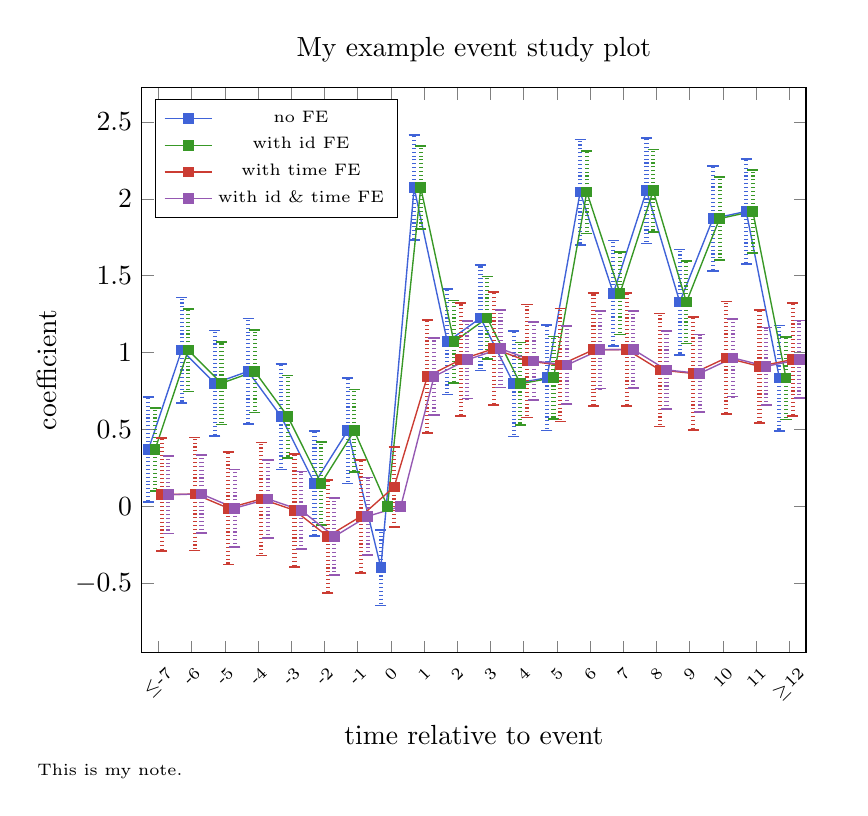
\begin{tikzpicture}
\begin{axis}[title={My example event study plot}, title style={}, xlabel={time relative to event}, xlabel style={}, ylabel={coefficient}, ylabel style={}, xticklabel style={font={\fontsize{6}{6}\selectfont}, rotate={45}}, yticklabel style={}, width={240pt}, height={204pt}, legend style={font={\fontsize{6}{6}\selectfont}, at={(0.02, 0.98)}, anchor={north west}}, symbolic x coords={$\leq$-7,-6,-5,-4,-3,-2,-1,0,1,2,3,4,5,6,7,8,9,10,11,$\geq$12}, xtick={$\leq$-7,-6,-5,-4,-3,-2,-1,0,1,2,3,4,5,6,7,8,9,10,11,$\geq$12}, xmin={{[normalized]-0.5}}, xmax={{[normalized]19.5}}, scale only axis]
    \addplot[mark={square*}, mark options={mark size={1.75pt}, line width={0pt}, fill={rgb,255: red, 64; green, 99; blue, 216}, fill opacity={1}, draw={rgb,255: red, 64; green, 99; blue, 216}, draw opacity={1}}, error bars/error mark={|}, error bars/error mark options={mark size={2.0pt}, solid, line width={0.6pt}, fill={rgb,255: red, 64; green, 99; blue, 216}, fill opacity={1}, draw={rgb,255: red, 64; green, 99; blue, 216}, draw opacity={1}}, error bars/error bar style={draw={rgb,255: red, 64; green, 99; blue, 216}, draw opacity={1}, densely dotted, line width={1.5pt}}, draw={rgb,255: red, 64; green, 99; blue, 216}, draw opacity={1}, line width={0.5pt}, error bars/y dir={both}, error bars/y explicit, x filter/.code={{\pgfmathadd{\pgfmathresult}{-0.30000000000000004}}}]
        coordinates {
            ($\leq$-7,0.36968848040224767) +- (0,0.34267)
            (-6,1.0161642543359581) +- (0,0.34267)
            (-5,0.8004351374649978) +- (0,0.34267)
            (-4,0.8778993522840808) +- (0,0.34267)
            (-3,0.5827695112478881) +- (0,0.34267)
            (-2,0.14944225350724832) +- (0,0.34267)
            (-1,0.49160731110003014) +- (0,0.34267)
            (0,-0.39846952781011685) +- (0,0.24537)
            (1,2.0726463666986965) +- (0,0.34267)
            (2,1.069919698272852) +- (0,0.34267)
            (3,1.2250710642968259) +- (0,0.34267)
            (4,0.797671985702108) +- (0,0.34267)
            (5,0.8364708751691308) +- (0,0.34267)
            (6,2.0437448807973797) +- (0,0.34267)
            (7,1.385907470897294) +- (0,0.34267)
            (8,2.052924230676942) +- (0,0.34267)
            (9,1.3283311252365637) +- (0,0.34267)
            (10,1.8713616815794547) +- (0,0.34267)
            (11,1.917987763924949) +- (0,0.34267)
            ($\geq$12,0.8338398361407332) +- (0,0.34267)
        }
        ;
    \addlegendentry {no FE}
    \addplot[mark={square*}, mark options={mark size={1.75pt}, line width={0pt}, fill={rgb,255: red, 56; green, 152; blue, 38}, fill opacity={1}, draw={rgb,255: red, 56; green, 152; blue, 38}, draw opacity={1}}, error bars/error mark={|}, error bars/error mark options={mark size={2.0pt}, solid, line width={0.6pt}, fill={rgb,255: red, 56; green, 152; blue, 38}, fill opacity={1}, draw={rgb,255: red, 56; green, 152; blue, 38}, draw opacity={1}}, error bars/error bar style={draw={rgb,255: red, 56; green, 152; blue, 38}, draw opacity={1}, densely dotted, line width={1.5pt}}, draw={rgb,255: red, 56; green, 152; blue, 38}, draw opacity={1}, line width={0.5pt}, error bars/y dir={both}, error bars/y explicit, x filter/.code={{\pgfmathadd{\pgfmathresult}{-0.10000000000000003}}}]
        coordinates {
            ($\leq$-7,0.36968848040220775) +- (0,0.26859)
            (-6,1.0161642543359184) +- (0,0.26859)
            (-5,0.8004351374649588) +- (0,0.26859)
            (-4,0.8778993522840413) +- (0,0.26859)
            (-3,0.5827695112478481) +- (0,0.26859)
            (-2,0.14944225350720935) +- (0,0.26859)
            (-1,0.4916073110999914) +- (0,0.26859)
            (0,0.0) +- (0,0.0)
            (1,2.0726463666986588) +- (0,0.26859)
            (2,1.069919698272813) +- (0,0.26859)
            (3,1.2250710642967875) +- (0,0.26859)
            (4,0.7976719857020685) +- (0,0.26859)
            (5,0.8364708751690915) +- (0,0.26859)
            (6,2.0437448807973415) +- (0,0.26859)
            (7,1.385907470897255) +- (0,0.26859)
            (8,2.0529242306769047) +- (0,0.26859)
            (9,1.3283311252365249) +- (0,0.26859)
            (10,1.8713616815794172) +- (0,0.26859)
            (11,1.917987763924911) +- (0,0.26859)
            ($\geq$12,0.8338398361406931) +- (0,0.26859)
        }
        ;
    \addlegendentry {with id FE}
    \addplot[mark={square*}, mark options={mark size={1.75pt}, line width={0pt}, fill={rgb,255: red, 203; green, 60; blue, 51}, fill opacity={1}, draw={rgb,255: red, 203; green, 60; blue, 51}, draw opacity={1}}, error bars/error mark={|}, error bars/error mark options={mark size={2.0pt}, solid, line width={0.6pt}, fill={rgb,255: red, 203; green, 60; blue, 51}, fill opacity={1}, draw={rgb,255: red, 203; green, 60; blue, 51}, draw opacity={1}}, error bars/error bar style={draw={rgb,255: red, 203; green, 60; blue, 51}, draw opacity={1}, densely dotted, line width={1.5pt}}, draw={rgb,255: red, 203; green, 60; blue, 51}, draw opacity={1}, line width={0.5pt}, error bars/y dir={both}, error bars/y explicit, x filter/.code={{\pgfmathadd{\pgfmathresult}{0.09999999999999998}}}]
        coordinates {
            ($\leq$-7,0.07645489065628541) +- (0,0.36715)
            (-6,0.07996822101712153) +- (0,0.36715)
            (-5,-0.011650219338167567) +- (0,0.36715)
            (-4,0.048274055401767546) +- (0,0.36715)
            (-3,-0.025795428786321184) +- (0,0.36715)
            (-2,-0.19579864129185204) +- (0,0.36715)
            (-1,-0.06466735007183605) +- (0,0.36715)
            (0,0.1268890275225385) +- (0,0.25962)
            (1,0.8447808240898919) +- (0,0.36715)
            (2,0.9532945471851118) +- (0,0.36715)
            (3,1.0256382459735534) +- (0,0.36715)
            (4,0.9454918497954898) +- (0,0.36715)
            (5,0.9192463471134921) +- (0,0.36715)
            (6,1.0183105850288388) +- (0,0.36715)
            (7,1.02004968243716) +- (0,0.36715)
            (8,0.8870106225498695) +- (0,0.36715)
            (9,0.8643245121103151) +- (0,0.36715)
            (10,0.965706757507417) +- (0,0.36715)
            (11,0.9105573459927425) +- (0,0.36715)
            ($\geq$12,0.9555153257114715) +- (0,0.36715)
        }
        ;
    \addlegendentry {with time FE}
    \addplot[mark={square*}, mark options={mark size={1.75pt}, line width={0pt}, fill={rgb,255: red, 149; green, 88; blue, 178}, fill opacity={1}, draw={rgb,255: red, 149; green, 88; blue, 178}, draw opacity={1}}, error bars/error mark={|}, error bars/error mark options={mark size={2.0pt}, solid, line width={0.6pt}, fill={rgb,255: red, 149; green, 88; blue, 178}, fill opacity={1}, draw={rgb,255: red, 149; green, 88; blue, 178}, draw opacity={1}}, error bars/error bar style={draw={rgb,255: red, 149; green, 88; blue, 178}, draw opacity={1}, densely dotted, line width={1.5pt}}, draw={rgb,255: red, 149; green, 88; blue, 178}, draw opacity={1}, line width={0.5pt}, error bars/y dir={both}, error bars/y explicit, x filter/.code={{\pgfmathadd{\pgfmathresult}{0.3}}}]
        coordinates {
            ($\leq$-7,0.07645489065630728) +- (0,0.25216)
            (-6,0.0799682210171434) +- (0,0.25216)
            (-5,-0.011650219338145695) +- (0,0.25216)
            (-4,0.048274055401789306) +- (0,0.25216)
            (-3,-0.025795428786298924) +- (0,0.25216)
            (-2,-0.19579864129182978) +- (0,0.25216)
            (-1,-0.06466735007181373) +- (0,0.25216)
            (0,0.0) +- (0,0.0)
            (1,0.8447808240899137) +- (0,0.25216)
            (2,0.9532945471851332) +- (0,0.25216)
            (3,1.0256382459735751) +- (0,0.25216)
            (4,0.9454918497955114) +- (0,0.25216)
            (5,0.9192463471135135) +- (0,0.25216)
            (6,1.0183105850288605) +- (0,0.25216)
            (7,1.0200496824371816) +- (0,0.25216)
            (8,0.8870106225498908) +- (0,0.25216)
            (9,0.8643245121103363) +- (0,0.25216)
            (10,0.9657067575074385) +- (0,0.25216)
            (11,0.9105573459927636) +- (0,0.25216)
            ($\geq$12,0.9555153257114926) +- (0,0.25216)
        }
        ;
    \addlegendentry {with id \& time FE}
\end{axis}
\newdimen\notewidth
                    \pgfextractx{\notewidth}{\pgfpointdiff{\pgfpointanchor{current bounding box}{west}}
                    {\pgfpointanchor{current bounding box}{east}}}\draw node[text width={\the\notewidth}, anchor={north west}, at={(current axis.outer south west)}, align={left}, font={\fontsize{6}{6}\selectfont}] {This is my note.};
\end{tikzpicture}
\end{document}
